\documentclass{iansnotes}

\title{Electrons and Photons}
\author{ian.mcloughlin@atu.ie}
\date{Last updated: \today}

\begin{document}
 
\maketitle


\section{Dividing Gold}
\begin{tikzpicture}[-latex, thick]
  \draw
    ( 0, 0) node (f)  {\includegraphics[width=40mm]{img/goldbar.png}}
    ( 6, 2) node (h1) {\includegraphics[width=20mm]{img/goldbar.png}}
    ( 6,-2) node (h2) {\includegraphics[width=20mm]{img/goldbar.png}}
    (10, 3) node (q1) {\includegraphics[width=10mm]{img/goldbar.png}}
    (10, 1) node (q2) {\includegraphics[width=10mm]{img/goldbar.png}}
    (10,-1) node (q3) {\includegraphics[width=10mm]{img/goldbar.png}}
    (10,-3) node (q4) {\includegraphics[width=10mm]{img/goldbar.png}};
  
  \draw  (f.east) edge node[above] {$\frac{1}{2}$} (h1.west)
         (f.east) edge node[below] {$\frac{1}{2}$} (h2.west)
        (h1.east) edge node[above] {$\frac{1}{4}$} (q1.west)
        (h1.east) edge node[below] {$\frac{1}{4}$} (q2.west)
        (h2.east) edge node[above] {$\frac{1}{4}$} (q3.west)
        (h2.east) edge node[below] {$\frac{1}{4}$} (q4.west);
\end{tikzpicture}


\section{Photoelectric Effect}
\begin{circuitikz}[
  lightwave/.style={draw=gray, decorate, decoration={expanding waves, angle=20}},
  lightbulb/.style={circle, fill=violet}
]
  \ctikzset{tubes/height=3, tubes/width=0.7};
  \draw (4,2) node[diodetube, rotate=-90] (vacc) {};
  \draw[lightwave] (5,3) node[lightbulb] {}  -- (vacc.tube bottom center);
  \draw (0,0) to[battery,invert] (8,0) to[ammeter] (8,2) to[short] (vacc.anode);
  \draw (vacc.cathode) to[short] (1,2) to[short] (0,2) to[short] (0,0);
\end{circuitikz}

\marginnote{\bibentry{photoelectriceffectbritannica}}

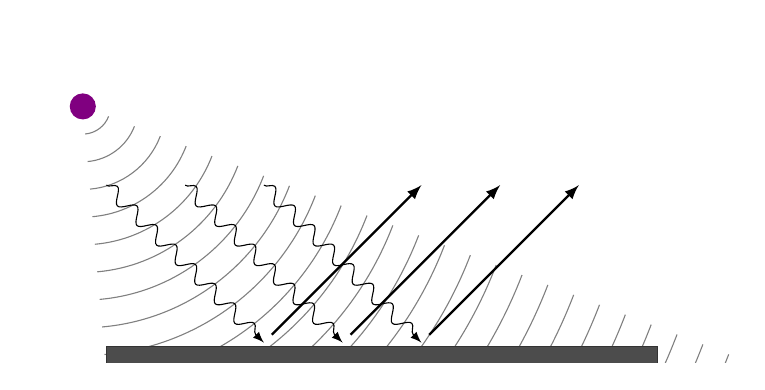
\begin{tikzpicture}[
  photon/.style={-latex,decorate,decoration={snake,post length=1mm}},
  electron/.style={-latex,thick},
  lightwave/.style={draw=gray, decorate, decoration={expanding waves, angle=32}},
  lightbulb/.style={circle, fill=violet},
  metalslab/.style={fill=black!70, draw=black!80}
]
  \clip (-1,-0.25) rectangle (8,4);
  \draw[lightwave] (-0.3,3) node[lightbulb] {}  -- ++(-53:10);
  \draw[metalslab] (0,-0.05) rectangle ++(7,-0.25) ;
  \draw[photon]   (0,2) -- (2,0);
  \draw[photon]   (1,2) -- (3,0);
  \draw[photon]   (2,2) -- (4,0);
  \draw[electron] (2.1,0.1) -- (4,2);
  \draw[electron] (3.1,0.1) -- (5,2); 
  \draw[electron] (4.1,0.1) -- (6,2);
\end{tikzpicture}


\section{Bohr Model}
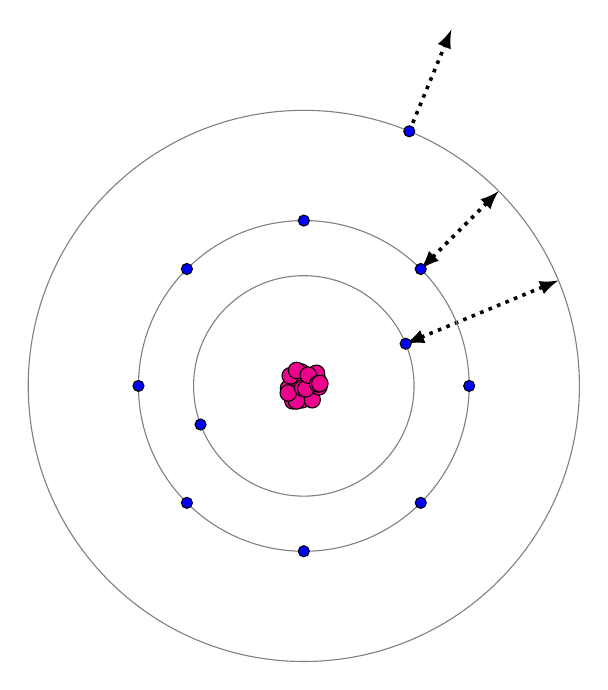
\begin{tikzpicture}[scale=0.7,
  transition/.style={latex-latex,line width=1.3pt,dotted,draw=black},
  orbit/.style={draw=gray},
  electron/.style={fill=blue},
  nucleus/.style={fill=cyan}
]
  \draw[transition] (45:3) -- (45:5);
  \draw[transition] (22.5:2) -- (22.5:5);
  \draw[transition,-latex] (67.5:5) -- (67.5:7);
  \draw[nucleus] (0,0) circle (0.25);
  \draw[orbit] (0,0) circle (2);
  \draw[orbit] (0,0) circle (3);
  \draw[orbit] (0,0) circle (5);
  \foreach \e in {22.5,200.5} \draw[electron] (\e:2) circle (0.1);
  \foreach \e in {0,45,90,...,315} \draw[electron] (\e:3) circle (0.1);
  \draw[electron] (67.5:5) circle (0.1);
  \foreach \x in {1,2,...,23}
    \draw[fill=magenta] (rand*0.3,rand*0.3) circle (0.15);
\end{tikzpicture} \\[8mm]

\noindent \includegraphics[width=50mm]{img/hydrogen_spectrum_2.jpg}

\marginnote[-55mm]{\bibentry{chemlibreh2spectrum}}

\vspace{10mm}

\section{Double Slit}
\begin{marginfigure}
  \includegraphics[width=50mm]{img/electron_double_slit.jpg}
  \caption*{Electrons}
\end{marginfigure} 

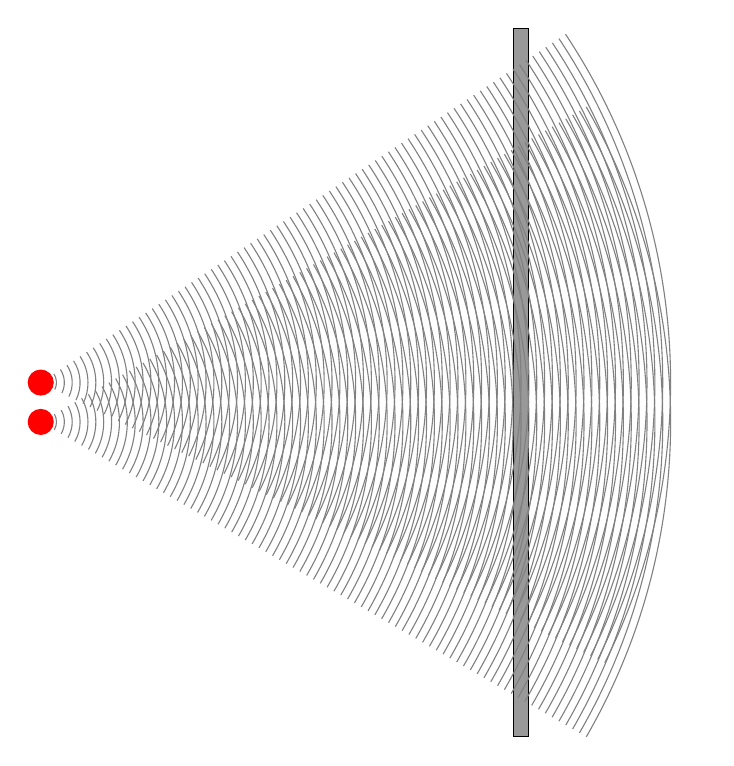
\begin{tikzpicture}[
  lightwave/.style={draw=gray, decorate, decoration={expanding waves, angle=30, segment length=1mm}},
  lightbulb/.style={circle, fill=red}
]
\draw[fill=black!40]            (6,-4) rectangle (6.2,5);
  \draw[lightwave] (0,0.5) node[lightbulb] {}  -- (8,1);
  \draw[lightwave] (0,0) node[lightbulb] {}  -- (8,0);
\end{tikzpicture}

\includegraphics[width=50mm]{img/double_single_slit.png}





\end{document}